%%%%%________________Section3_________________________%%%%

\section{Cadre théorique}
La notation de \textbf{Kndall-Lee} permet de décrire de grandes familles de systèmes de files d'attente \cite{QS_K}.
\subsection{Notation de Kendall-Lee}
On décrit les systèmes de file d'attente à l'aide de  six attributs: $$x_1/x_2/x_3/x_4/x_5/x_6.$$
La première caractéristique précise la nature du \textbf{processus d'arrivée}. On utilise les abréviations standard suivantes:
\newl \begin{tabular}{p{0.25cm}p{0.25cm}p{15cm}}
$M$ &$=$& intervalles d’arrivées exponentiels \\ & & \quad   indépendants et identiquement distribués (iid) \\
$D$ &$=$& intervalles d’arrivées déterministes, iid\\
$E_{k}$ &$=$& intervalles d’arrivées suivent Erlang $\mathcal{E}(R,k)$, iid  \\
$G$ &$=$& intervalles d’arrivées iid et régis par  \\ & & \quad une distribution générale.
\end{tabular}
\newl
La deuxième caractéristique précise la nature du \textbf{temps de service}:
\newline \newline
\begin{tabular}{p{0.25cm}p{0,25cm}p{12cm}}
$M$ &$=$& temps de services exponentiels, iid \\
$D$ &$=$& temps de services déterministes, iid\\
$E_{k}$ &$=$& temps de services Erlang $\mathcal{E}(R,k)$, iid \\
$G$ &$=$& temps de service iid et régis par  \\ & & \quad une distribution générale.
\end{tabular}
\newpage\noindent
La troisième caractéristique représente le \textbf{nombre de ser\-veurs parallèles}; c'est un nombre entier positif. \newl  La quatrième caractéristique décrit la \textbf{politique de service}:
\newl
\begin{tabular}{ccc}
FCFS &$=$& premier arrivé, premier servi\\
LCFS &$=$& dernier arrivé, dernier servi\\
SIRO &$=$& service dans un ordre aléatoire\\
GD &$=$& politique de service générale.
\end{tabular}
\newl
La cinquième caractéristique précise le \textbf{nombre maximal d’utilisateurs} pouvant être accommodés par le système, tandis que la sixième caractéristique  donne le \textbf{taille de la population} dont sont issus les utilisateurs. À moins que le nombre de clients potentiels ne soit du même ordre de grandeur que le nombre de serveurs, la taille de la population est considérée comme infinie. \newl Dans de nombreux modèles importants, $x_4/x_5/x_6$ correspond à $\textrm{GD}/\infty/\infty$; dans ce cas, ces attributs sont souvent omis de la description de la file d'attente.\newl  Par exemple, $M/M/3/\textrm{FCFS}/20/\infty$ pourrait représenter une banque avec 3 guichets, des temps d'arrivée et de service exponentiels, une politique de service ``premier arrivé, premier servi'', une capacité totale de 20 clients et un bassin de population infini dans lequel puiser. La situation est partiellement illustrée à la Figure~\ref{fig:1}.
\begin{figure}[t]
	\centering
		\includegraphics[width=0.49\textwidth]{Images/fig1Queue_\ldoc.png}
	\caption{\small Une file d'attente avec $3$ guichets  -- $M/M/3/\textrm{FCFS}/20/\infty$.}
	\label{fig:1}
\end{figure}
\subsection{Processus de naissance et de mort}
\begin{figure}[!t]
	\centering
		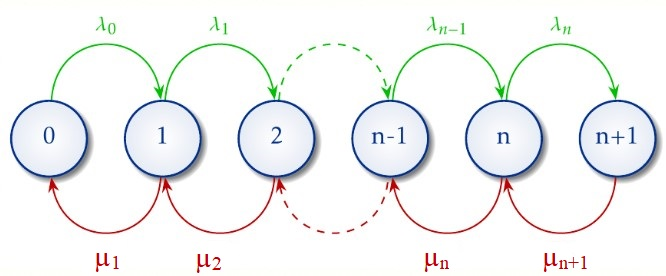
\includegraphics[width=0.49\textwidth]{Images/fig2Queue.jpg}
	\caption{\small Processus de naissance et de mort; les taux de natalité et de mortalité sont indiqués par $\lambda_n$ et $\mu_m$, respectivement (source inconnue).}
	\label{fig:2}\hrule
\end{figure}
L'\textbf{état} d'un système de file d’attente au temps $t$ est le nombre de clients dans le système de file d’attente (soit en attente en ligne ou en service) au temps $t$. Lorsque $t = 0$, l'état du système est tout simplement le nombre initial de clients dans le système.  Cet état vaut la peine d'être noté car il affecte l'état du système pour les autres instants $t$.  \par En conséquence, nous définissons $P_{i,j} (t)$ comme la probabilité que l'état soit $j$ au temps $t$, étant donné que l'état à $t = 0$ était $i$. Pour des valeurs élevées de $t$, $P_{i,j} (t)$ devient indépendant de $i$ et se rapproche d'une limite $\pi_{j}$. Cette limite est le \textbf{régime stable} de l’état $j$.\newl Il est en général difficile de déterminer les étapes des arrivées et des services qui mènent à un état stable $\pi_j$. De même, à partir d'un $t$ près du début, il est difficile de déterminer exactement quand un système atteindra son état stable $\pi_j$, et même si un tel état existe. \par Par souci de simplicité, lorsqu'on étudie un système de file d'attente, on commence par supposer que l'état d'équilibre a déjà été atteint.\newl  
Un \textbf{processus de naissance et de mort} est un processus de Markov dans lequel les états sont indexés par des entiers non négatifs, et les transitions d’états ne sont autorisées qu'entre états ``voisins.'' Après une ``naissance,'' l'état du système passe de $n$ à $n+1$; après une ``mort,'' de $m$ à $m-1$. En général, les taux de natalité et de mortalité sont représenté spar $\lambda_n$ et $\mu_m$, respectivement (comme on peut le constater à la Figure~\ref{fig:2}). Les processus de nature  \textbf{purement naissance} sont ceux pour lesquels $\mu_m=0$ pour tout $m$; pour ceux de nature \textbf{purement mort}, on a $\lambda_n=0$ pour tout $n$. La \textbf{solution d'état stable} d'un processus de naissance-mort, c'est-à-dire la probabilité $\pi_n$ que le système se retrouve dans l'état $n$, \textit{peut} en fait être calculée: 
\begin{align} \pi_{n} &= \pi_{0}\frac{\lambda_{0} \lambda_{1} \cdots \lambda_{n-1}}{\mu_{1} \mu_{2} \cdots \mu_{n}},\quad  \text{pour    } n=1,2,\cdots,\label{eq:ssbr}
\end{align}
où $\pi_{0}$ est la probabilité que le système se retrouve dans l'état 0 (c’est-à-dire sans utilisateurs). On peut également montrer \cite{QS_K1} que:
$$ \pi_{0} = \frac{1}{1+ \sum^{\infty}_{n=1} \prod^{n-1}_{j=0} \frac{\lambda_{j}}{\mu_{j+1}}}.$$ 

\subsection{Loi de Little}
Les analystes et les clients souhaitent souvent déterminer combien temps l'utilisateur moyen passe dans le système de file d'attente. Soit $W$ le \textbf{temps d'attente prévu passé dans le système de file d’attente}, y compris le temps passé dans la file et le temps de service, et $W_{q}$ le \textbf{temps d'attente prévu d'un client dans la file}. Les deux valeurs $W$ et $W_{q}$ sont calculés en supposant que l'état d'équilibre du système a été atteint. En utilisant un puissant résultat connu sous le nom de \textbf{loi de Little}, $W$ et $W_{q}$ sont facilement liés au nombre de clients dans la file d'attente et à ceux qui font la queue. \newl  Pour tout système de file d'attente (ou tout sous-ensemble d'un système de file d'attente), on considère les quantités suivantes:
\begin{itemize}[noitemsep]
\item $\lambda = $  le nombre moyen d'arrivées dans le système par unité de temps;  
\item $L =$  le nombre moyen d'utilisateurs présents dans le système de file d'attente;
\item $L_{q} = $  le nombre moyen d'utilisateurs qui font la queue;
\item $L_{s} = $  le nombre moyen d'utilisateurs en service;
\item $W = $  le temps moyen qu'un utilisateur passe dans le système de file d'attente;
\item $W_{q} = $  le temps moyen qu'un utilisateur passe dans la file d'attente, et
\item $W_{s} = $  le temps moyen qu'un utilisateur passe en service.
\end{itemize}
Les utilisateurs du système ne peuvent que se trouver dans la file d'attente ou en service, de sorte que $L = L_{q} + L_{s}$ et $W = W_{q} + W_{s}$ (dans ces définitions, toutes les moyennes sont des moyennes de régime permanent (``steady-state’’)). Pour la plupart des systèmes de file d'attente dans lesquels un tel régime existe, la loi de Little se résume par 
\begin{align*}
L &=  \lambda W, \quad L_{q} = \lambda W_{q}, \quad\mbox{et}
\quad L_{s}= \lambda W_{s}.
\end{align*}
\begin{Exemple} Si, en moyenne, 46 clients entrent dans un restaurant à chaque heure où il est ouvert, et s'ils passent, en moyenne, 10 minutes à attendre d'être servis, nous devrions nous attendre à ce que $46\cdot 1/6 \approx 7.7$ clients se retrouve dans la file d'attente à tout moment, en moyenne. \end{Exemple}

